%!TEX root = elastic_3d_sbp.tex
\subsubsection{Iterative methods}\label{iterative_section}
In the proposed scheme (\ref{coarse_scheme})--(\ref{traction_continuous_curvi}), we need to solve a $3n_1^cn_2^c\times 3n_1^cn_2^c$ linear system at each time step twice for the continutiy of the traction force along the interface (\ref{traction_gamma_pre}) and (\ref{traction_gamma_corr}). Even ethough we can do LU factorization one time before the time loop start and reuse it at each time step, it is very expensive to do LU factorization for a large problem. Besides, consider solving real problems which are usually in large scale, we want to perform the computation on many processors on a parallel distributed memory machine, but it is not clear how to calculate the LU factorization of a matrix on many processors. 

In this paper, we propose three iterative methods: block Jacobian method, conjugate gradient method, preconditioned conjugate gradient method. We find that preconditioned conjugate gradient method is the most efficient one and conjugate gradient method needs most iteration numbers.

For the problem proposed in Section \ref{manufactured_sol}, the structure of the coefficient matrix of the linear system (\ref{traction_continuous_curvi}) is shown in Figure \ref{Mass_matrix} which is determined by the interplation operator $\mathcal{P}$ and restriction operator $\mathcal{R}$. We choose the red circles in the purple circles in Figure \ref{Mass_matrix} to be the block Jacobian matrix in block Jacobian iterative method and pre-conditioning matrix in pre-conditioned conjugate gradient iterative method. We also set a absolute error tolerance $1e-7$ for each iterative method.

\begin{table}[htb]
	\begin{center}
		\begin{tabular}{|c|c c c|}
			\hline
			$h^c_k = 2h^f_k$   & ~~~~ CG ~~~~& Block Jacobian & Preconditioned CG  \\
			\hline
			$2\pi/24$ &37.76& 24.96& 4.07\\
			\hline
			$2\pi/48$ &38.61 & 25.38 & 2.88\\
			\hline 
			$2\pi/96$ &39.14 &25.43 & 2.55\\
			\hline
		\end{tabular}
	\end{center}
	\caption{condition number of matrices in conjugate gradient method, block Jacobian method, preconditioned conjugate gradient method}\label{condition_number}
\end{table} 
Table \ref{condition_number} shows the condition number of the original coefficient matrix, the block Jacobian matrix and the coefficient matrix after applying pre-conditioner respectively. We observe that the condition number for preconditioned conjugate gradient method is smallest which is consistent with the results for iteration number of different iterative methods : there is around $44$ iterations for conjugate gradient method, $13$ iterations for block Jacobian method and $9$ iterations for preconditioned conjugate method.

\begin{figure}[H]
	\centering
	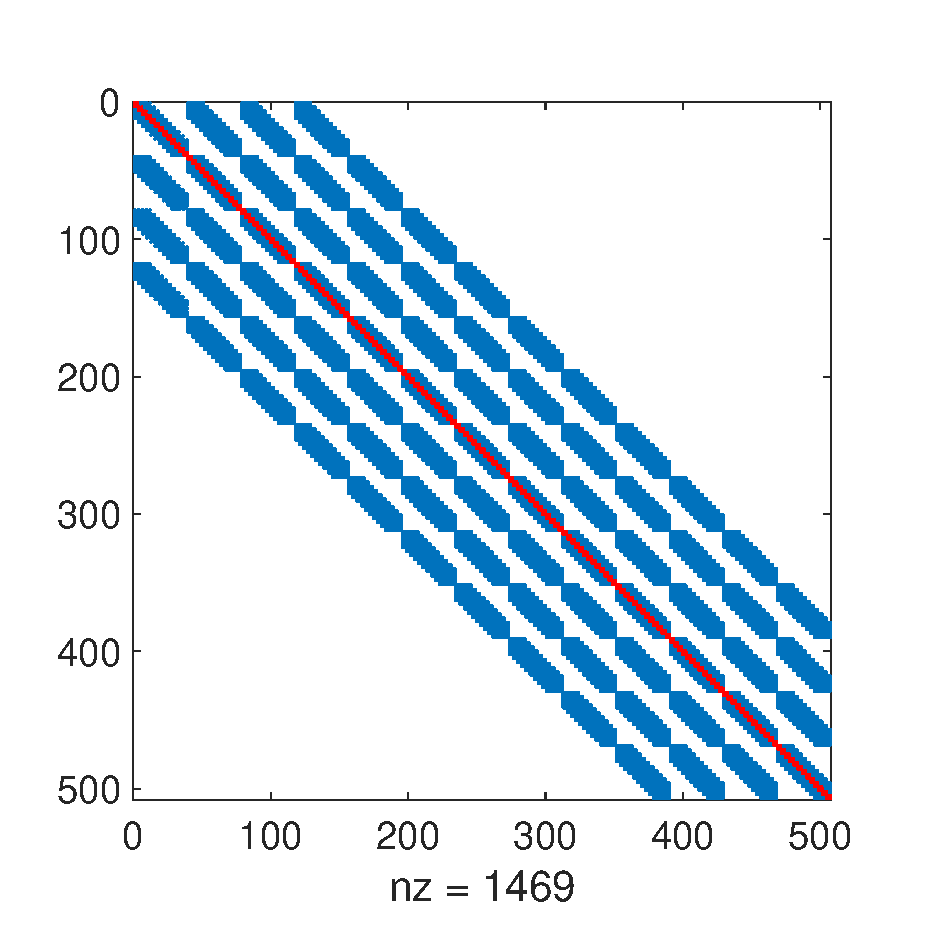
\includegraphics[width=0.45\textwidth]{Mass_matrix.eps}
	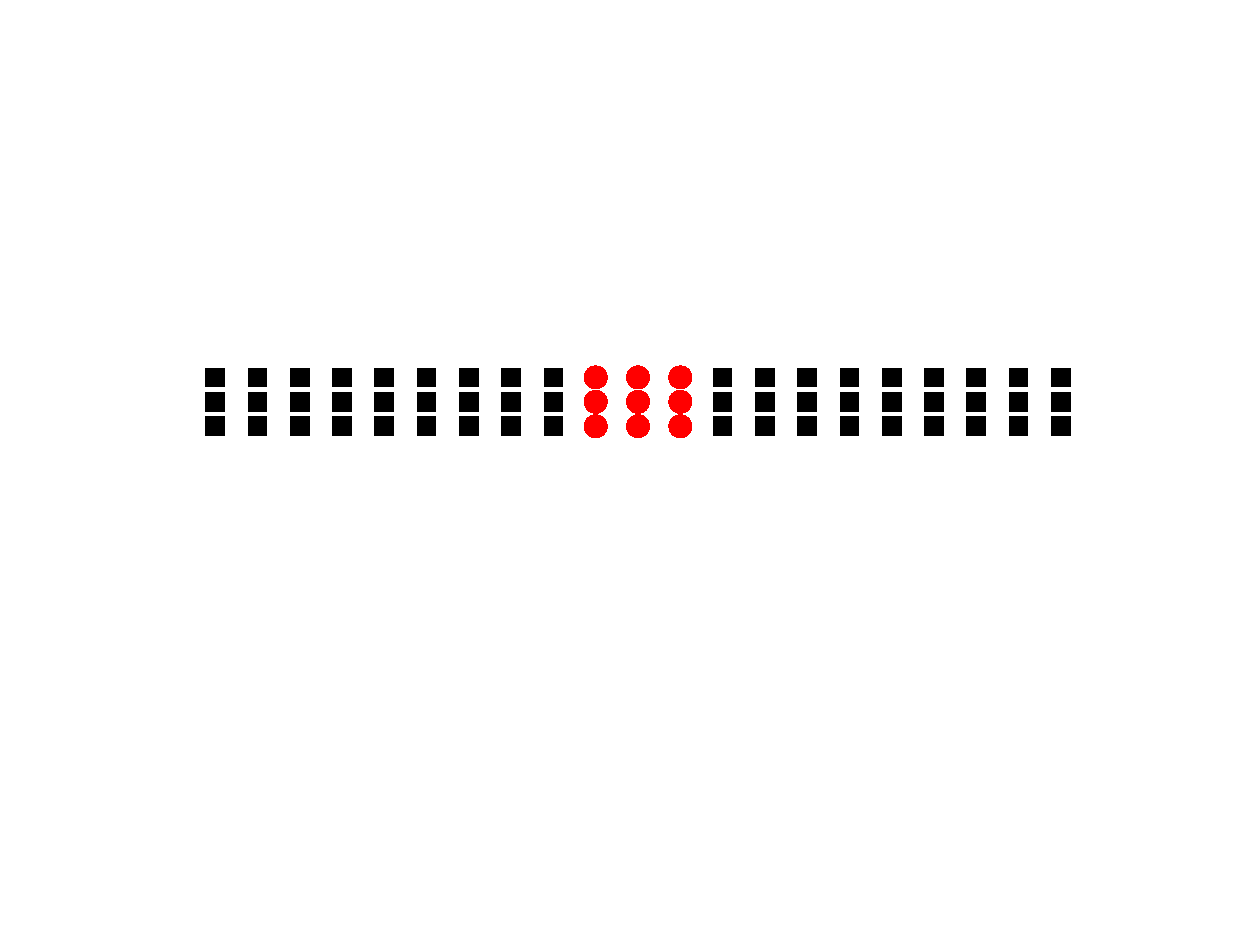
\includegraphics[width=0.45\textwidth]{Mass_block_diagonal.eps}
	\caption{\scriptsize{The left are the structure of the coefficient matrix of the linear system (\ref{traction_continuous_curvi}). For each triangle and circle in the left, it has the structure as in the right.}}\label{Mass_matrix}
\end{figure}
